\documentclass{article}
\usepackage[utf8]{inputenc}

\title{Homework 3}
\author{Benny Chen}
\date{September 28, 2022}

\usepackage{color}
\usepackage{amsthm}
\usepackage{amssymb} 
\usepackage{amsmath}
\usepackage{listings}
\usepackage{xcolor}
\usepackage{listings}
\usepackage{graphicx}
\usepackage{tabularx}
\usepackage[hidelinks]{hyperref}

\lstdefinelanguage[mips]{Assembler}{%
  % so listings can detect directives and register names
  alsoletter={.\$},
  % strings, characters, and comments
  morestring=[b]",
  morestring=[b]',
  morecomment=[l]\#,
  % instructions
  morekeywords={[1]abs,abs.d,abs.s,add,add.d,add.s,addi,addiu,addu,%
    and,andi,b,bc1f,bc1t,beq,beqz,bge,bgeu,bgez,bgezal,bgt,bgtu,%
    bgtz,ble,bleu,blez,blt,bltu,bltz,bltzal,bne,bnez,break,c.eq.d,%
    c.eq.s,c.le.d,c.le.s,c.lt.d,c.lt.s,ceil.w.d,ceil.w.s,clo,clz,%
    cvt.d.s,cvt.d.w,cvt.s.d,cvt.s.w,cvt.w.d,cvt.w.s,div,div.d,div.s,%
    divu,ecall,eret,floor.w.d,floor.w.s,j,jal,jalr,jr,l.d,l.s,la,lb,lbu,%
    ld,ldc1,lh,lhu,li,ll,lui,lw,lwc1,lwl,lwr,madd,maddu,mfc0,mfc1,%
    mfc1.d,mfhi,mflo,mov.d,mov.s,move,movf,movf.d,movf.s,movn,movn.d,%
    movn.s,movt,movt.d,movt.s,movz,movz.d,movz.s,msub,msubu,mtc0,mtc1,%
    mtc1.d,mthi,mtlo,mul,mul.d,mul.s,mulo,mulou,mult,multu,mulu,mv,neg,%
    neg.d,neg.s,negu,nop,nor,not,or,ori,rem,remu,rol,ror,round.w.d,%
    round.w.s,s.d,s.s,sb,sc,sd,sdc1,seq,sge,sgeu,sgt,sgtu,sh,sle,%
    sleu,sll,sllv,slt,slti,sltiu,sltu,sne,sqrt.d,sqrt.s,sra,srav,srl,%
    srlv,sub,sub.d,sub.s,subi,subiu,subu,sw,swc1,swl,swr,syscall,teq,%
    teqi,tge,tgei,tgeiu,tgeu,tlt,tlti,tltiu,tltu,tne,tnei,trunc.w.d,%
    trunc.w.s,ulh,ulhu,ulw,ush,usw,xor,xori},
  % assembler directives
  morekeywords={[2].align,.ascii,.asciiz,.byte,.data,.double,.extern,%
    .float,.globl,.half,.kdata,.ktext,.set,.space,.text,.word},
  % register names
  morekeywords={[3]\$0,\$1,\$2,\$3,\$4,\$5,\$6,\$7,\$8,\$9,\$10,\$11,%
    \$12,\$13,\$14,\$15,\$16,\$17,\$18,\$19,\$20,\$21,\$22,\$23,\$24,%
    \$25,\$26,\$27,\$28,\$29,\$30,\$31,%
    \$zero,\$at,\$v0,\$v1,\$a0,\$a1,\$a2,\$a3,\$t0,\$t1,\$t2,\$t3,\$t4,
    \$t5,\$t6,\$t7,\$s0,\$s1,\$s2,\$s3,\$s4,\$s5,\$s6,\$s7,\$t8,\$t9,%
    \$k0,\$k1,\$gp,\$sp,\$fp,\$ra},
}[strings,comments,keywords]

\definecolor{CommentGreen}{rgb}{0,.6,0}
\lstset{
  language=[mips]Assembler,
  escapechar=@, % include LaTeX code between `@' characters
  keepspaces,   % needed to preserve spacing with lstinline
  basicstyle=\small\ttfamily\bfseries,
  commentstyle=\color{CommentGreen},
  stringstyle=\color{cyan},
  showstringspaces=false,
  keywordstyle=[1]\color{blue},    % instructions
  keywordstyle=[2]\color{magenta}, % directives
  keywordstyle=[3]\color{red},     % registers
}

\begin{document}

\maketitle

\section*{Question 1}
Translate function foo() in the following C code to RISC-V assembly code. Assume function
bar() has already been implemented. The constraints/tips are:
\begin{enumerate}
    \item Allocate register s1 to sum, and register s2 to i.
    \item There are no load or store instructions in the loop. If we want to preserve values across
        function calls, place the value in a saved register before the loop. For example, we keep
        variable i in register s2.
    \item Identify the registers that are changed in function foo() but should be preserved. Note that
        the callee, bar(), may change any temporary and argument registers
    \item Save registers at the beginning of the function and restore them before the exit.    
\end{enumerate}
Your code should follow the flow of the C code. Write concise comments.
Clearly mark instructions for saving registers, loop, function calls, restoring register, etc.

\begin{center}
    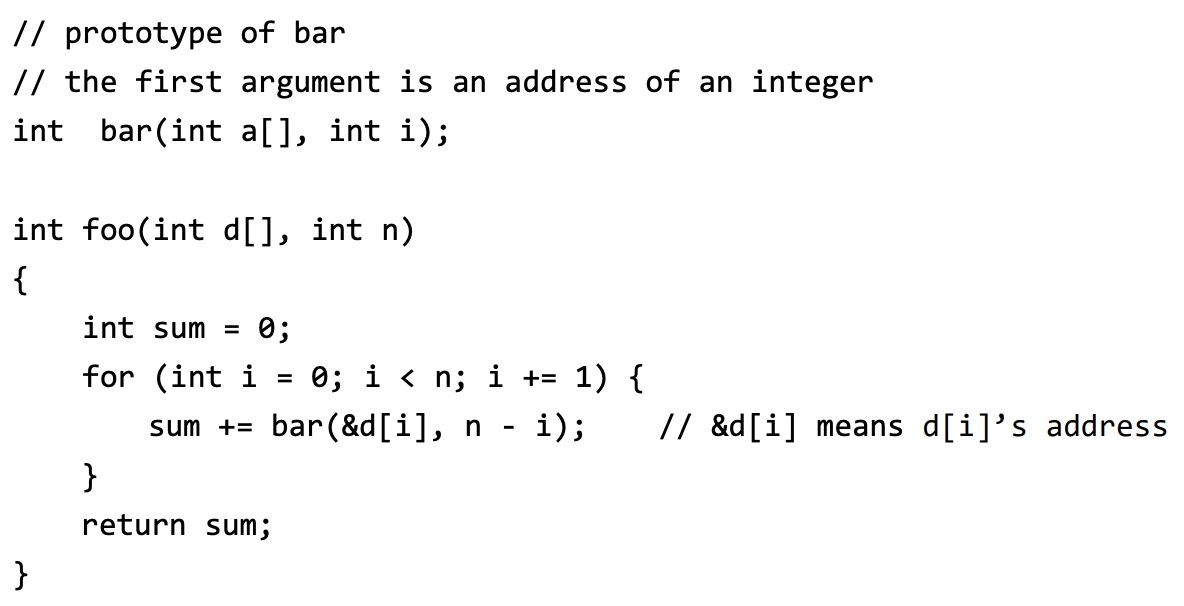
\includegraphics[scale=.55]{images/Q1.png}
\end{center}

\textbf{Answer:}
\begin{lstlisting}
    foo:
	addi	sp,sp,-20 #Allocate space 
	sw	s1,0(sp)
	sw	s2,4(sp)
	sw	s3,8(sp)
	sw	s4,12(sp)
	sw	ra,16(sp)
	
	addi	s1,s1,0 #s1 = sum = 0
	addi	s2,s2,0 #s2 = i = 0
	addi	s3,s3,0 #s3 = d address = ? 
	addi	s4,s4,100 #s4 = n = ? 
	
loop:	
	slli	a0,s2,2 #offset of i
	add	a0,a0,s3 #&d[i]
	sub	a1,s4,s2 #n-i
	jal	ra,bar #bar(&d[i],n-i)
	
	add	s1,s1,a0 #sum += output of bar(&d[i],n-i)
	
	addi	s2,s2,1 #i+=1
	blt	s2,s4,loop #if i < n

return:
	addi	a0,s1,0 #foo returns sum so into a0

	#restore all
	lw	s1,0(sp)
	lw	s2,4(sp)
	lw	s3,8(sp)
	lw	s4,12(sp)
	lw	ra,16(sp)
	
	addi	sp,sp,20
	
	jr ra
\end{lstlisting}

\section*{Question 2}
Translate function msort() in the following C code to RISC-V assembly code. Assume
merge() and copy() are already implemented. The array passed to msort() has at most 256
elements.
Your code should follow the flow of the C code. Write concise comments. Clearly mark
instructions for saving registers, function calls, restoring register, and so on.
To make the code easier to read, we change sp twice at the beginning of the function: once
for saving registers and once for allocating memory for array c.
The function should have only one exit. There is only one return instruction.
Another reminder: callees may change any temporary and argument registers.

\begin{center}
    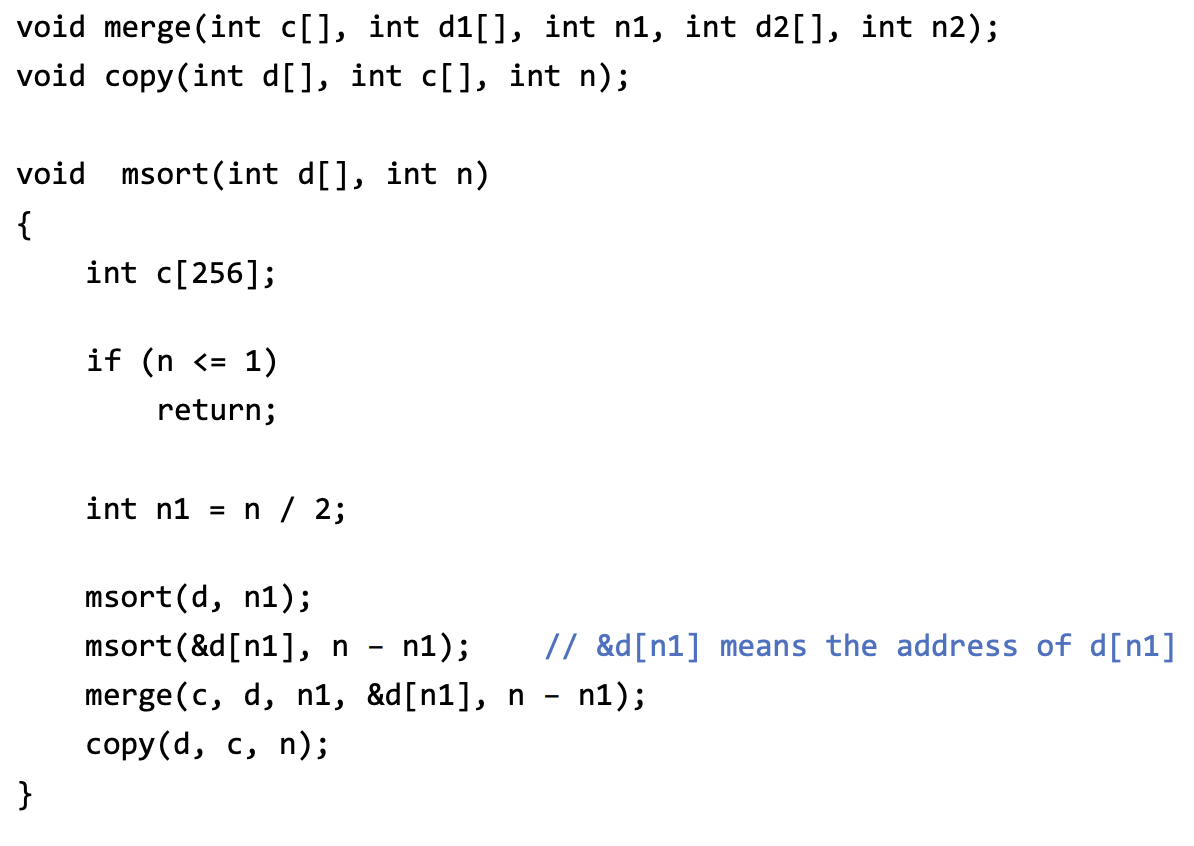
\includegraphics[scale=.55]{images/Q2.png}
\end{center}

\textbf{Answer:}
\begin{lstlisting}
# merge inputs in (c[], d1[], n1, d2[], n2)
# copy inputs in (d[], c[], n)

# Inputs in d[] and int n
msort:
	addi	sp,sp,-1036 #allocate space for variables
	
	sw	ra,1032(sp)
	sw	s2,1028(sp)
	sw	s1,1024(sp) 
	
	addi	s1,a0,0 #Save D[] to s1
	addi	s2,a1,0 #Save n to s2
	
	addi	t0,t0,2 # t0 = 2 for if statement
	blt		a1,t0,exit # return if n < 2

	srai	t1,s2,1 # n1 = n/2
	addi	a1,t1,0 # a1 = n1
	jal     ra,msort  # call msort(d,n1)
	
	slli	t3,t1,2 #t3 = n1 * 4
	add     a0,t3,s1 #n1 + &d = &d[n1] = a0
	sub     a1,s2,t1 #n-n1 = a1
	jal     ra,msort  # call msort(&d[n1], n - n1)
	
	addi    a0,sp,0 #c
	addi    a1,s1,0 #d
	addi    a2,t1,0 #n1
	add     a3,t3,s1 #n1 + &d = &d[n1] = a3
	sub     a4,s2,t1 #n-n1 = a4
	jal     ra,merge #merge(c, d, n1, &d[n1], n - n1)
	
	addi	a0,s1,0 #d
	addi	a1,sp,0 #c
	addi	a2,s2,0 #n
	jal     ra,copy #copy(d, c, n)
	
exit:
	#restore registers
	lw      s1,1024(sp) 
	lw      s2,1028(sp)
	lw      ra,1032(sp)
	
	addi    sp,sp,1036 
	
	jr      ra
\end{lstlisting}

\section*{Question 3}
Find the machine code for the following instruction. Assume all instructions are labeled
sequentially, for example, I1, I2, I3, …, I150. 

\begin{center}
    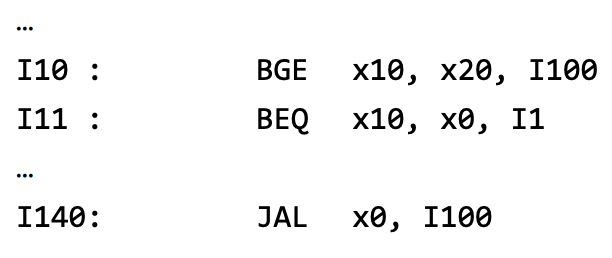
\includegraphics[scale=.75]{images/Q3.png}
\end{center}

\subsection*{I10:   BGE x10,x20,I100}

Opcode: 1100011\\
funct3: 101\\
Type: SB\\
rs1: 01010\\
rs2: 10100\\
work: (100 - 10) * 4 = 360\\
immediate: 0000101101000\\
Machine code: 0001011 10100 01010 101 01000 1100011\\
Hex: 0x17455463\\

\begin{center}
	\begin{tabularx}{1.15\textwidth} { 
		| >{\centering\arraybackslash}X 
		| >{\centering\arraybackslash}X 
		| >{\centering\arraybackslash}X 
		| >{\centering\arraybackslash}X
        | >{\centering\arraybackslash}X
		| >{\centering\arraybackslash}X | }
	   \hline
	   	im[12][10:5] & rs2 & rs1 & funct3 & im[4:1][11] & Opcode \\
	   \hline
	   0001011  & 10100  & 01010 & 101 & 01000 & 1100011 \\
	  \hline
	\end{tabularx}
\end{center}

\subsection*{I11:   BEQ x10,x0,I1}

Opcode: 1100011\\
funct3: 000\\
Type: SB\\
rs1: 01010\\
rs2: 00000\\
work: (1 - 11) * 4 = -40\\
immediate: 1111111011000\\
Machine code: 1111110 00000 01010 000 11001 1100011\\
Hex: 0xFC050CE3\\

\begin{center}
    \begin{tabularx}{1.15\textwidth} { 
        | >{\centering\arraybackslash}X 
        | >{\centering\arraybackslash}X 
        | >{\centering\arraybackslash}X 
        | >{\centering\arraybackslash}X
        | >{\centering\arraybackslash}X
        | >{\centering\arraybackslash}X | }
       \hline
       	im[12][10:5] & rs2 & rs1 & funct3 & im[4:1][11] & Opcode \\
       \hline
       1111110  & 00000  & 01010 & 000 & 11001 & 1100011 \\
      \hline
    \end{tabularx}
\end{center}

\subsection*{I140:   JAL x0,I100}

Opcode: 1101111\\
Type: UJ\\
rd: 00000\\
work: (100 - 140) * 4 = -160\\
immediate: 111111111111101100000\\
Machine code: 11110110000111111111 00000 1101111\\
Hex: 0xF61FF06F\\

\begin{center}
    \begin{tabularx}{1.15\textwidth} { 
        | >{\centering\arraybackslash}X 
        | >{\centering\arraybackslash}X 
        | >{\centering\arraybackslash}X | }
       \hline
        imm[20][10:1][11][19:12] & rd & Opcode \\
       \hline
       11110110000111111111 & 00000 & 1101111 \\
      \hline
    \end{tabularx}
\end{center}

\newpage

\section*{Question 4}

Decode the following instructions in machine code. Find the offset in decimal and then the
target address in hexadecimal. The hexadecimal number before the colon is the instruction’s
address.

\begin{center}
    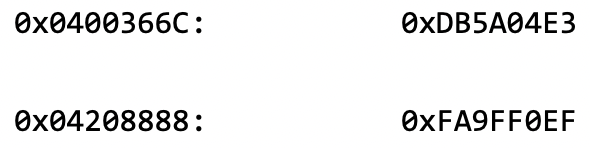
\includegraphics[scale=.75]{images/Q4.png}
\end{center}

\subsection*{0x0400366C: 0xDB5A04E3}

Instruction in Binary: 1101101 10101 10100 000 01001 1100011\\
Opcode: 1100011\\
funct3: 000\\
Type: SB\\
rs1: 10100\\
rs2: 10101\\
immediate work: [1][1][101101][0100][0]\\
immediate: 1110110101000\\
Decimal: -600\\
Target address: 0x0400366C - 0x258 = 0x4003414\\
Instruction: BEQ x20,x21,0x4003414\\

\subsection*{0x04208888: 0xFA9FF0EF}

Instruction in Binary: 11111010100111111111 00001 1101111\\
Opcode: 1101111\\
Type: UJ\\
rd: 00001\\
immediate work: [1][11111111][1][1111010100][0]\\
immediate: 111111111111110101000\\
Decimal: -88\\
Target address: 0x04208888 - 0x58 = 0x4208830\\
Instruction: JAL x1,0x4208830\\

\end{document}